\documentclass{article}
\usepackage[utf8]{inputenc}
\title{MATH 20C Notes - Week Six}
\author{C-Rin}
\date{October 2019}

\usepackage{natbib}
\usepackage{graphicx}
\usepackage{gensymb}
\usepackage{amsmath}
\usepackage{amssymb}
\usepackage{wrapfig}
\usepackage{diffcoeff}
\usepackage{microtype}

\graphicspath{ {./images/} }

\begin{document}

\maketitle

\section*{Introduction}
Deep 

\begin{figure}[h!]
\centering
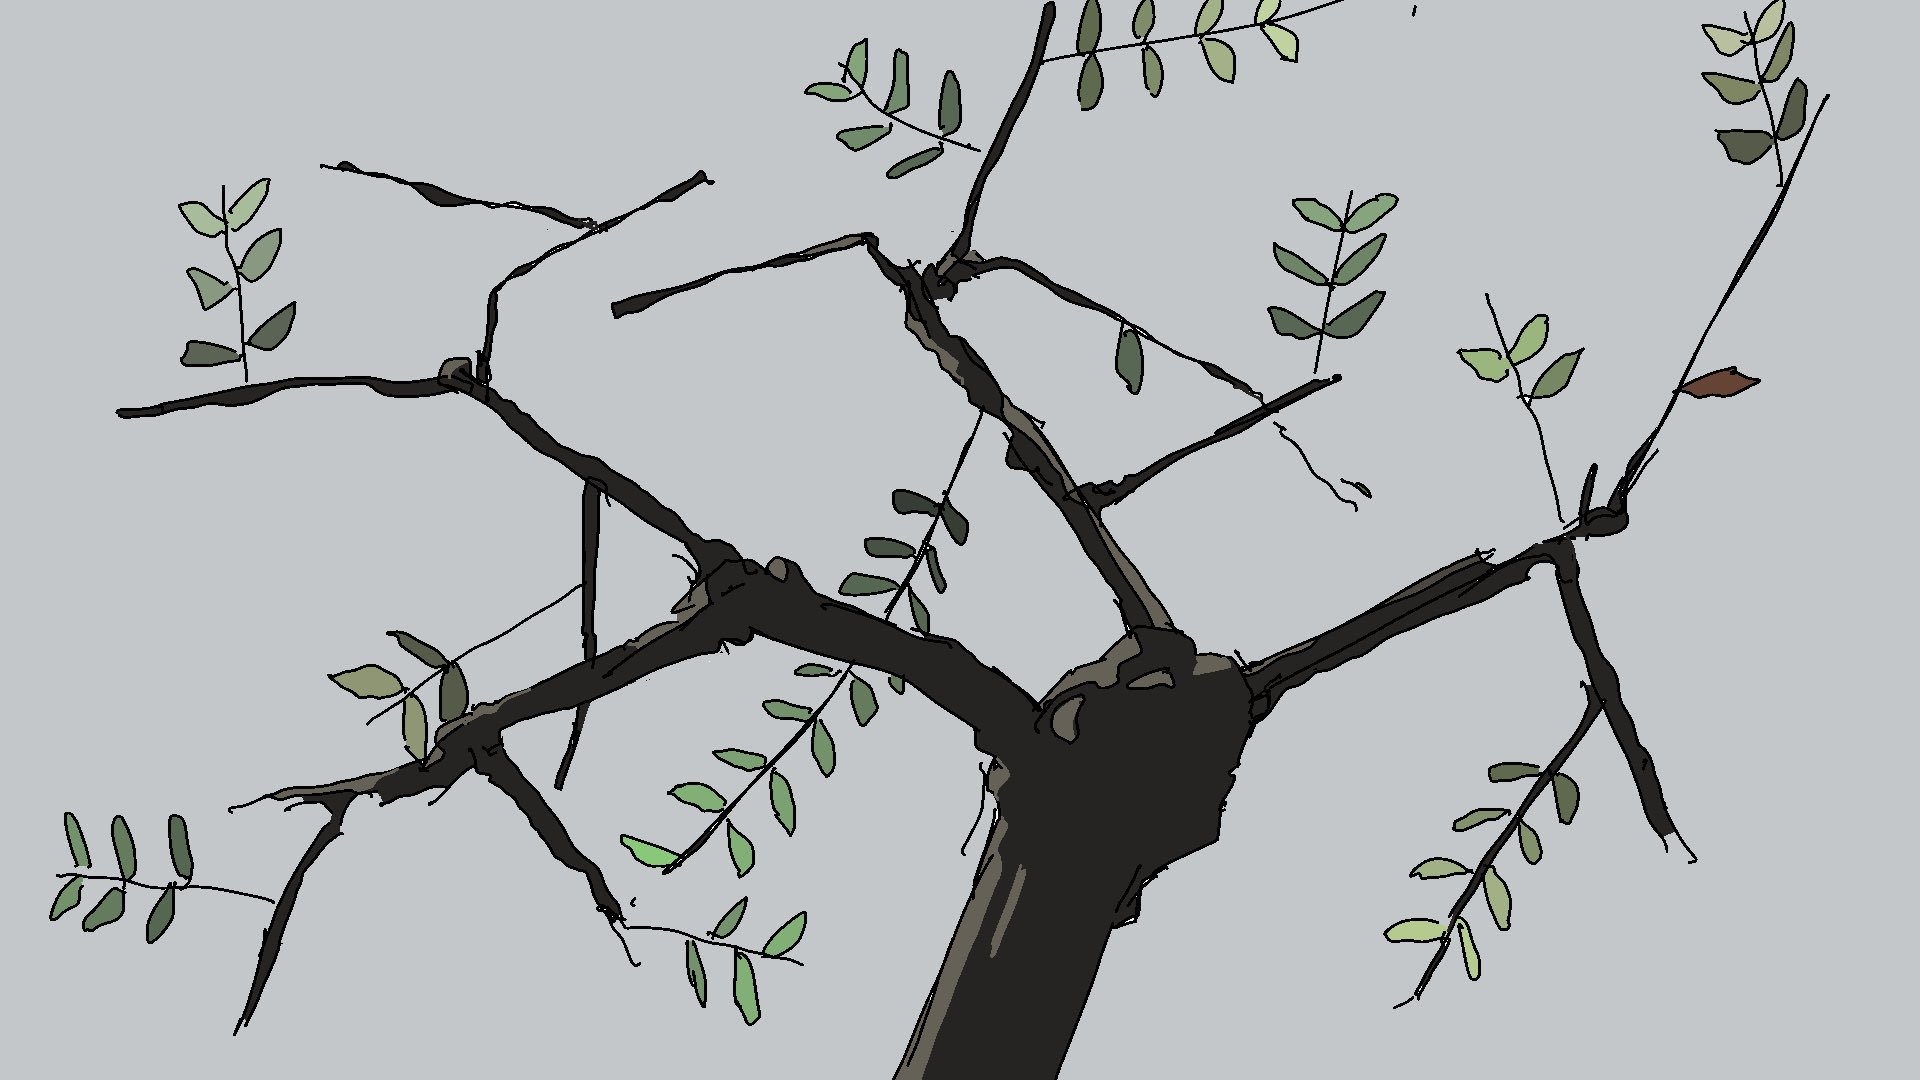
\includegraphics[scale=0.1]{tree.jpg}
\caption{A stylized tree (unspecified species)}
\end{figure}


\section{Acceleration/Newton's 2nd Law}

Let $\bar{c}:\mathbb{R}\rightarrow\mathbb{R}^3$ be a differentiable path (a particle's position at time (t)).

The velocity of $\bar{c}$ is 
\[\bar{c}\prime (t) = (\frac{\partial x}{\partial t},\frac{\partial y}{\partial t}\frac{\partial z}{\partial t})\]

The speed is the magnitude $||\bar{c}\prime (t)||$

The acceleration is $\bar{c}\prime\prime(t)=(x\prime\prime(t),y\prime\prime(t),z\prime\prime(t))$

\subsection{Differentiation Rules for Paths}
Let $\bar{b}:\mathbb{R}\rightarrow\mathbb{R}^3$ and $\bar{c}:\mathbb{R}\rightarrow\mathbb{R}^3$ be differentiable paths.

Let $p(t)$ be a scalar function

\subsubsection*{Product Rules}
\begin{enumerate}
    \item Sum Rule
        \[\frac{\partial}{\partial t}(\bar{b}(t)+\bar{c}(t))=\bar{b}\prime(t)+\bar{c}\prime(t)\]
    \item Dot Product Rule
        \[\frac{\partial}{\partial t}(\bar{b}(t)\cdot\bar{c}(t))=\bar{b}\prime(t)\cdot\bar{c}(t)+\bar{c}\prime(t)\cdot\bar{b}(t)\]
    \item Scalar Product Rule
        \[\frac{\partial}{\partial t}(p(t)\cdot\bar{c}(t))=p\prime(t)\bar{c}(t)+p(t)\bar{c}\prime(t)\]
    \item Cross Product Rule
        \[\frac{\partial}{\partial t}(\bar{b}(t)\times\bar{c}(t))=\bar{b}\prime(t)\times\bar{c}(t)+\bar{c}\prime(t)\times\bar{b}(t)\]
\end{enumerate}

\subsection*{Example}
Suppose 
\[\bar{b}(t)=(\sin(t),\cos(t),0)\]
\[\bar{c}(t)=(0,t,t^2)\]

\[\bar{b}(t)\times\bar{c}(t)=(t^2\cos(t),-t^2\sin(t),t\sin(t))\]

\[\frac{\partial}{\partial t}(\bar{b}\times\bar{c})=(2t\cos(t)-t^{2}\sin(t),-2t\sin(t))-t^2\cos(t),sin(t)+t\cos(t)\]
\[\bar{b}\prime(t) = (\cos(t),-\sin(t),0)\qquad \bar{c}\prime(t)=(0,1,2t)\]

\[\bar{b}\prime\times\bar{c}+\bar{b}\times\bar{c}\prime=(-t^2\sin(t),-t^2\cos(t), t\cos(t))+(2t\cos(t),-2t\sin(t),t\sin(t))\]

\subsection*{Newton's Second Law}
\[\bar{F}=m\bar{a}\]

\subsection*{Exercise}
Suppose there is a particle with initial position
\[\bar{r}(0)=(6,-2,1)\qquad \bar{v}(0)=(-5,1,3)\qquad\bar{a}(t)=(2,-6,-4)\]

Find the trajectory/path of the particle.

\[\int a(t)=v(t) = (2t,-6t,-4t)+c\qquad v(0)=(-5,1,3)=(0,0,0)\]
\[v(t)=(2t-5,-6t+1,-4t+3)\]
\[\int v(t)=r(t)=(t^2-5t,-3t^2+t,-2t^2+3t)+c\]
\[r(0)=(6,-2,1)=(0,0,0)\]
\[r(t)=(t^2-5t+6,-3t^2+t-2,-2t^2+3t+1)\]


\section{Arc Length}
Consider a path 
\[\bar{c}: [a,b]\rightarrow\mathbb{R}^3\]

This path traces out a curve, and the length of that curve is the arc length.

\[L=\int^{b}_{a} ||c\prime(t)|| dt \qquad \bar{c}(t)=(x(t),y(t),z(t))\]

\[\int \sqrt{x\prime(t)^2+y\prime(t)^2+z\prime(t)^2}dt\]

\subsection*{Example - Deriving the Circumference of a circle}

\begin{wrapfigure}{r}{0.2\textwidth}
    \begin{center}
      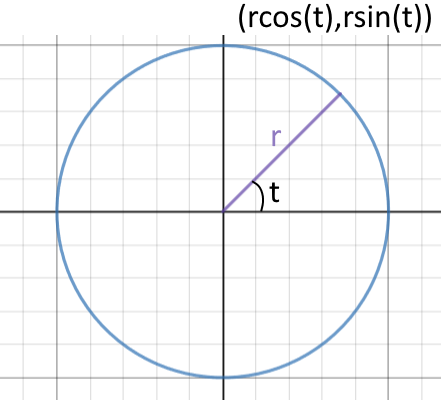
\includegraphics[width=0.40\textwidth]{unitCircle.png}
    \end{center}
\end{wrapfigure}
$t$ is in $[0,2\pi]$ and the arc length is $2\pi r$

\[\int_{0}^{2\pi} \sqrt{(-r\sin(t))^2+(rcos(t))^2}dt\]
\[=\int_{0}^{2\pi} \sqrt{r^{2}\sin^2(t)+r^2\cos^{2}(t)}dt\]
\[=\int_{0}^{2\pi} \sqrt{r^{2}(\sin^{2}t+\cos^2(t))}dt\]
\[=\int_{0}^{2\pi} \sqrt{r^{2}(1)}dt = \int_{0}^{2\pi} rdt\]
=\[=2\pi r\]
\newpage
\subsection*{Example}


\begin{wrapfigure}{r}{0.2\textwidth}
    \begin{center}
      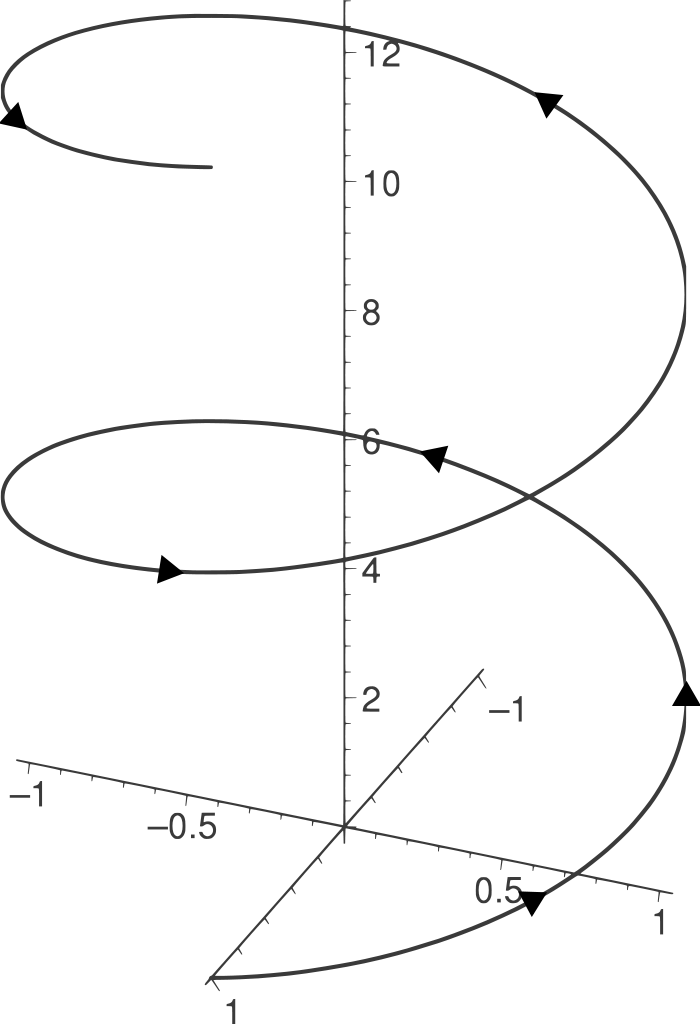
\includegraphics[width=0.30\textwidth]{Helix.png}
    \end{center}
\end{wrapfigure}


\[\bar{c}(t)=(t,\cos(t),\sin(t))\qquad 0\leq t\leq 2\pi\]
\[x\prime(t)=1\]
\[y\prime(t)=-\sin(t)\]
\[z\prime(t)=\cos(t)\]
\[=\int_{0}^{2\pi} \sqrt{2}dt\]
\[=2\pi \sqrt{2}\]

\subsection*{Exercise}
Find the length of the curve
\[\bar{c}(t)=(2t,\frac{4}{3}t^{\frac{3}{2}},\frac{1}{2}t^2)\mbox{  for  } 0\leq t\leq 3\]
\[x\prime(t)=2\qquad y\prime(t)=2\sqrt{t}\qquad z\prime(t)=t\]
\[\int^{3}_{0} \sqrt{4+4t+t^2}dt = \int_{0}^{3} \sqrt{(t+2)^2}dt=\int_{0^{3}}(t+2)dt\]
\[
    \left[ \frac{t^2}{2} + 2t \right]^{3}_{0}=\frac{9}{2}+6=\frac{21}{2}
\]

\subsection*{Remark}
Arc length can be computed in any dimension

Let $\bar{c}:[a,b]\rightarrow\mathbb{R}^n$

Arc length $= \int^{b}_{a} ||\bar{b}\prime(t)||dt$

\[\int^{b}_{a} x\prime (t) dt = x(b)-x(a)\]

\newpage
\section{Double Integral}
\subsection*{The Intuitive Meaning}
\[f:\mathbb{R}^2\rightarrow\mathbb{R}\]
(Which takes values greater than $0$

\begin{figure}[h!]
    \centering
    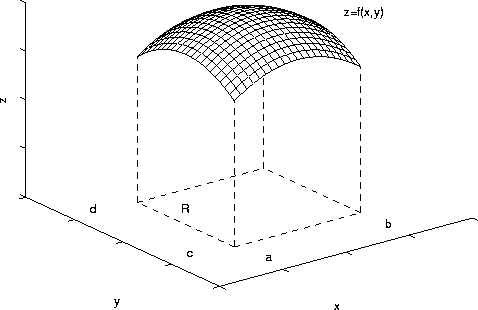
\includegraphics[scale=.5]{plot1.png}
    \caption{}
    \label{}
\end{figure}

The volume contained above $a\leq x \leq b$ and $c\leq y \leq d$

and below $z=f(x,y)$
\[\underbrace{=\int^{b}_{a}\int^{d}_{c} f(x,y)dy dx}_{\mbox{Double Integral}}\]

\subsection*{Example}
What is the volume of $z=z-x$ on the rectangular region of $0\leq x \leq 2$ and $0 \leq y \leq 3$
\[=\int^{2}_{0}\int^{3}_{0} (2-x)dy dx =\frac{2\cdot 2\cdot 3}{2}=6\]

\subsection*{Remark}
If we are integrating over a more interesting region, we can represent it as
\[\iint f(x,y)dydx\]

How in practice do we compute these volumes?

We can use Cavalieri's Principle to calculate the volume using cross sectioned areas where
\[\mbox{Volume }= \int^{a}_{b} A(x)dx\]

\subsection*{Example}
\[\int^1_0\int^1_0 (x^2+y^2)dxdy\]
Suppose $x$ is fixed (i.e. a constant) on $0\leq x \leq 1$

\[A(x)=\int^1_0 x^2+y^2 dy=\left[x^2 y+\frac{1}{3}y^3\right]^1_0 =x^2+\frac{1}{3}\]
\[\int^1_0 x^2+\frac{1}{3}dx = \frac{x^3}{3}+\frac{1}{3}x=\frac{1}{3}+\frac{1}{3}=\frac{2}{3}\]

\subsection*{Intuitive Definition of Integrals in 2D}
$f:\mathbb{R}^2\rightarrow\mathbb{R}$ with nonnegotiable values

\[int^{b}_{a}\int^{d}_{c} f(x,y)dydx = \mbox{the volume of the solid}\]
\begin{enumerate}
    \item bounded below by $\mathbb{R}$
    \item bounded by the graph $z=f(x,y)$
\end{enumerate}
We use iterative integrals to find the volume.

\[\underbrace{\int^b_a A(x)dx=int^{b}_{a}\int^{d}_{c} f(x,y) dy dx}_{Iterative Integral}\]


\end{document}